\chapter{Algoritmo de Conciliación.}\label{cap:capitulo4}

En esta sección, se introduce el Algoritmo de Conciliación basado en Agentes explicado en \cite{algoritmo}, se explicarán los diferentes pasos de la ejecución del algoritmo, así como un análisis de los resultados que aporta y las conclusiones que se pueden extraer de los mismos.



\section{Introducción al Algoritmo de Conciliación.}

A partir del etiquetado propio de un usuario, que refleja su propio conjunto de conceptos sobre los documentos, se pueden obtener diferentes resultados con dos de las principales herramientas del AFC: el retículo de conceptos y las bases Stem; mostrando la heterogeneidad semántica, que se ha descrito en capítulos anteriores. Desde el punto de vista de la navegación por medio de etiquetas, la heterogeneidad semántica hace que esta actividad no asegure el éxito de la misma. De este modo, para asegurar un uso eficiente de las etiquetas de otros usuarios, se debe poner en marcha algún razonador sobre estas etiquetas, cuyo fin es lograr un consenso (también representado por herramientas AFC), que permita la navegación entre estructuras de conceptos diferentes. En este escenario, es importante tratar de delegar estas tareas en agentes inteligentes, como se representa en la figura~\ref{fig:smaGeneral}.

\begin{figure}[t]
\centering
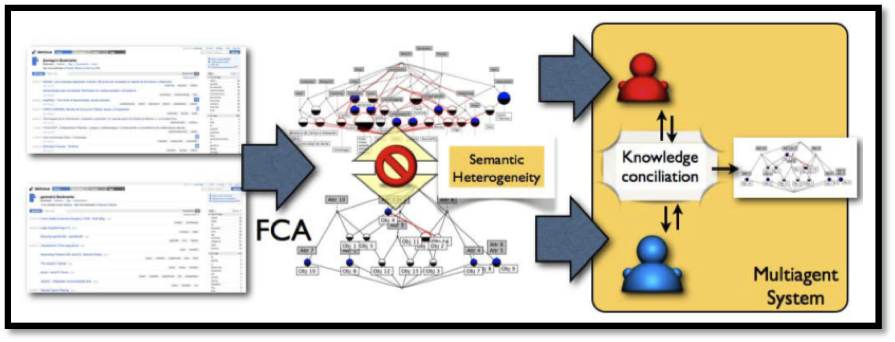
\includegraphics[scale=0.9]{img/4/smaGeneral}
\caption{Conciliación de conceptos a través de retículos de conceptos.
\label{fig:smaGeneral}}
\end{figure}


El Algoritmo original, que se describe detalladamente en \cite{algoritmo}, fue realizado en JADE (consultar más referencias sobre esta herramienta en \cite{jade}). JADE es una herramienta de Sistemas MultiAgente realizada en Java. Dado que en el presente trabajo, el SMA también se ha implementado en JADE, se usará este mismo sistema para la implementación de este algoritmo, de forma que el proceso de integración del algoritmo dentro del SMA sea más sencillo.






\section{Proceso de Conciliación.}

En esta sección se detallan los diferentes pasos (esquematizados en la figura~\ref{fig:algoritmo}) que se llevan a cabo en el algoritmo. Estos pasos son secuenciales; es decir, no se realiza el paso $n$ hasta haber finalizado el paso $n-1$ ($0< n \leq 6$).

\begin{figure}[t]
\centering
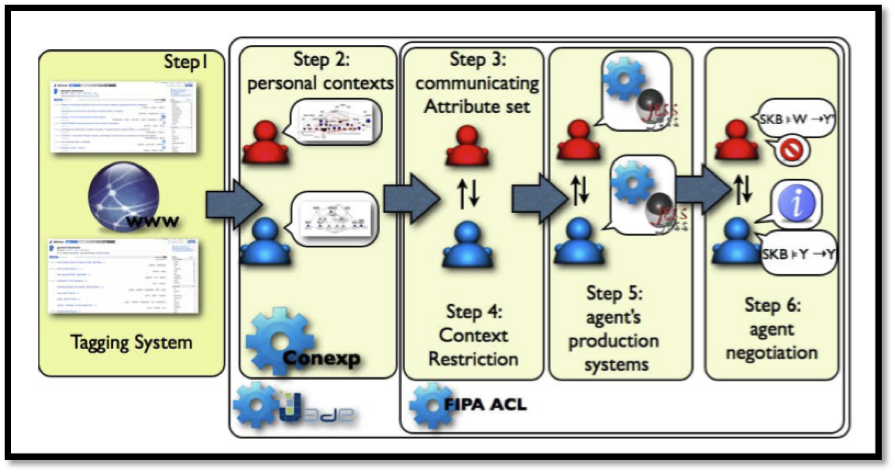
\includegraphics[scale=0.8]{img/4/algoritmo}
\caption{Algoritmo de conciliación
\label{fig:algoritmo}}
\end{figure}


\subsection{Paso 1: Creación de los Agentes.}

En este primer paso de inicialización, se crean a ambos agentes, de forma que éstos representan a los dos usuarios a lo que se les va a conciliar su conocimiento.

Para ello, cada agente deberá conocer los datos del usuario de Delicious al que representa ($id$ y $username$). Igualmente, deberá conocer el nombre del otro agente, con el que realizará la conciliación.

\subsection{Paso 2: Construcción del Contexto Formal y las Bases Stem.}

En este paso, los agente trabajan de forma paralela, sin interacciones entre ellos. Inicialmente, cada agente cargará su propio Conocimiento Base (KB). Este KB se construye a partir de la información de Delicious del usuario al que el agente representa, de forma que los objetos son las enlaces (URLs) y los atributos son las etiquetas asociadas a éstos.

Con estos datos, se construye el Contexto Propio del usuario, del cual se pueden extraer los Conceptos Formales así como las Bases Stem (SB). Para ello, se ha integrado en el algoritmo, la herramienta $Concept Explorer$ de $ConExp$ (ver \cite{conexp} para más referencias), que provee todos los algoritmos de AFC necesarios para realizar estos cálculos.

\subsection{Paso 3: Inicialización del Diálogo.}

En este paso se produce una doble tarea comunicativa, para iniciar el diálogo con el otro agente y comenzar, así, la Conciliación de sus conocimientos.

Por una parte, el agente debe enviar su propio Lenguaje (conjunto de atributos) al otro agente. Por otra, el agente se prepara para recibir el mismo tipo de mensaje del otro agente; es decir, el Lenguaje del otro usuario.

En el proceso de comunicación, se ajustará la intención de cada mensaje a las diferentes performativas FIPA y sus significados. De esta forma, el envío de los lenguajes se realizará con mensajes de performativa tipo {\tt INFORM}.

\subsection{Paso 4: Restricciones del Contexto Formal Propio.}

Después de esta breve comunicación, el agente debe calcular su Contexto Reducido. Para ello, primeramente calculará el Lenguaje Común; es decir, el conjunto de atributos que ambos usuarios comparten, y restringe su Contexto Formal a ese Lenguaje Común. Esta restricción también implica que muchos objetos de este contexto sean eliminados, debido a que no estén etiquetados con ninguna etiqueta de este Lenguaje Común.

Con este nuevo contexto, es decir, el Contexto Reducido propio del agente, éste calculará sus nuevo Retículo de Conceptos y las Bases Stems asociados a él.

\subsection{Paso 5: Creación del Sistema de Producción a partir de las Bases Stem.}

A partir de las Bases Stem calculadas en el paso anterior, el agente únicamente considera aquellas reglas cuyo soporte es mayor que cero. A este conjunto de implicaciones las llamaremos \emph{Bases Stem Kernel} (SKB).

Basándose en las SKB, se creará un sistema de producción, que servirá posteriormente para sugerir a otros agentes los cambios de los objetos que pueden ser aceptados en el contexto común. Este sistema de producción (usado para las nuevas sugerencias de etiquetas) ha sido implementado completamente, por los pocos requisitos del motor de inferencia, y porque no valía la pena integrarlo con otros motores, como Jess4\footnote{\url{http://www.jessrules.com/}} o Drools5\footnote{\url{http://www.jboss.org/drools}}.

\subsection{Paso 6: Negociación del Conocimiento entre Agentes.}

Finalmente, se lleva a cabo este proceso de comunicación y negociación, que se realiza limpiamente en un entorno multiagente. Aunque se podría haber implementado una comunicación cíclica o alternando cambios, mucho más asíncrona; este algoritmo elige la filosofía de multiagentes. La razón es que un escenario normal se compone de KB de diferentes tamaños (de los agentes), por lo que el proceso de comunicación para cada conciliación será diferente.

El proceso de negociación es el siguiente:

\begin{itemize}
	\item La negociación comienza con la creación, por cada agente, de un nuevo contexto (Contexto Común) donde se almacenará el conocimiento común y producirá los resultados de la conciliación. Además, se realiza un envío masivo de todos los objetos (incluidas sus etiquetas asociadas) al otro agente, y espera la respuesta para cada uno de estos objetos. Todos estos mensajes se describen con la performativa {\tt PROPOSE}.
	\item Cuando un agente recibe un objeto, comprueba inicialmente que este objeto satisface todas las implicaciones del SKB propio del agente, y en ese caso, lo incluye en el Contexto Común. Además envía un mensaje de aceptación al otro agente (performativa {\tt ACCEPT\_PROPOSAL}), para que éste también lo incluya en su contexto común.
	\item Si el objeto no satisface alguna implicación del SKB, se introduce en un sistema de producción, creado a partir del SKB (paso 5), y comprueba si alguno de los atributos obtenidos se puede añadir al objeto para que sea aceptado por el SKB. Este nuevo objeto se le envía al otro agente como “objeto nuevo”, reiniciando la negociación sobre dicho objeto. Si el sistema de producción no devuelve ninguna sugerencia, se elimina el objeto y se envía un mensaje de rechazo (performativa {\tt REJECT\_PROPOSAL}) al otro agente para que también lo elimine.
	\item Una vez que se realiza el proceso completo de intercambio de mensajes y  las negociaciones han terminado, los agentes tendrán un Contexto Común, que será igual para ambos agentes. Por tanto, se pueden extraer Conceptos y sugerencias de sus Bases Stem. Éstas representan una conceptualización compartida.
\end{itemize}


\section{Resultados y Conclusiones.}

El algoritmo anterior concilia el Conocimiento asociado a un par de usuarios de algún Sistema de Etiquetado. El método está basado en Análisis Formal de Conceptos, y está diseñado mediante tecnología Multiagente, mediante el cual los agentes colaboran para establecer una representación del conocimiento común, con un nuevo conjunto de etiquetado y nuevos retículos de conceptos.

Hay que indicar que el nuevo Contexto Común obtenido estará formado por el conjunto de atributos comunes (Lenguaje común). Sin embargo, el conjunto de objetos de este contexto estará formado por todos aquellos objetos, de cualquiera de los dos usuarios, que o bien satisfagan todas las implicaciones del Contexto particual de cada usuario, o bien generen nuevos atributos, a partir del Sistema de Producción, para que estas implicaciones acepten esta nueva etiquetación.

Según los datos empíricos aportados en \cite{algoritmo}, se puede concluir que la Conciliación entre dos usuarios genera un Contexto Común dónde el número de atributos (Lenguaje Común) es mucho menor, mientras que el número de objetos es mucho mayor que el de los Contextos Reducidos de cada usuario, ya que se aceptan objetos de ambos.



\begin{figure}[t]
  \begin{minipage}[b]{0.45\linewidth}\centering
	\begin{tabular}{l c c}
	\hline
	Usuario & jborrego & garanda \\ \hline
	Lenguaje & 351 & 137 \\ \hline
	Enlaces & 358 & 536 \\ \hline
	\end{tabular}
  \end{minipage}
\hspace{0.5cm}
   \begin{minipage}[b]{0.45\linewidth}
    \centering
	\begin{tabular}{l c c}
	\hline
	Usuario & jborrego & garanda \\ \hline
	Lenguaje & \multicolumn{2}{c}{19} \\ \hline
	Enlaces & 131 & 114 \\ \hline
	Implicaciones & 11 & 11 \\ \hline
	\end{tabular}
   \end{minipage}
\caption{Contextos antes (izq.) y después (der.) de reducir al Lenguaje Común.}
\label{fig:tabla1}
\end{figure}

\begin{figure}[t]\centering
	\begin{tabular}{l c}
	\hline
	 & Conciliación \\ \hline
	Lenguaje & 19 \\ \hline
	Enlaces & 245 \\ \hline
	Implicaciones & 121 \\ \hline
	\end{tabular}
\caption{Contexto Conciliado.}
\label{fig:tabla2}
\end{figure}

En el experimento realizado en \cite{algoritmo} se usan los usuarios de Delicious de los autores; es decir: {\em garanda}\footnote{http://delicious.com/garanda/} y {\em jborrego}\footnote{http://delicious.com/jborrego/}. Los Contextos iniciales de cada usuario se puede ver en la figura~\ref{fig:tabla1}, así como los Contextos Reducidos obtenidos. Tras aplicar el Algoritmo de Conciliación a estos contextos, se obtiene un Contexto Común, cuyos detalles se adjuntan en la figura~\ref{fig:tabla2}

